\chapter{Sprint 3 : Couche d'intelligence}

\section{Introduction}
Le Sprint~3 a doté \nova{} de sa couche d'intelligence~:
remplissage automatique de créneaux vides, apprentissage des
durées de consultation, vérificateur d'interactions
médicamenteuses, profils de véhicules pour garages, surprises
d'anniversaire, file d'attente en temps réel pour laboratoire,
avatars vocaux, assistant vocal et observation patient. Chacune
de ces fonctionnalités s'inscrit dans le modèle de pack sectoriel
qui permet d'activer ou de désactiver un domaine sans toucher au
reste du produit.

\section{Backlog du Sprint 3}
Le Sprint~3 ferme les \emph{user stories} de différenciation et
active les packs sectoriels.

\begin{table}[H]
  \centering\small
  \caption{Backlog du Sprint 3 : user stories et effort estimé.}
  \label{tab:bk-s3}
  \renewcommand{\arraystretch}{1.4}
  \begin{tabular}{|p{1.4cm}|>{\raggedright\arraybackslash}p{9.5cm}|>{\centering\arraybackslash}p{2.0cm}|}
    \hline\hline
    \textbf{ID} & \textbf{User story (résumé)} & \textbf{Effort (j)} \\
    \hline
    US10 & Campagnes vouchers d'anniversaire.                & 1,5 \\
    \hline
    US11 & Approbation des campagnes Demand-Fill.            & 2   \\
    \hline
    US12 & Auto-ajustement de durée de service.              & 2   \\
    \hline
    US14 & Consultation du dossier médical patient.          & 1,5 \\
    \hline
    US15 & Gestion des véhicules (garage).                   & 2   \\
    \hline
    US16 & QR de réception laboratoire.                      & 1,5 \\
    \hline
    US25 & Envoi photo des dégâts voiture.                   & 1   \\
    \hline
    US26 & Scan QR de réception (file d'attente).            & 1   \\
    \hline
    US27 & Position et ETA en file d'attente.                & 1   \\
    \hline
    US28 & Voucher anniversaire WhatsApp.                    & 1   \\
    \hline
    US33 & Scan quotidien Demand-Fill.                       & 1,5 \\
    \hline
    US34 & Batch anniversaire.                               & 1   \\
    \hline
    US35 & Apprentissage hebdomadaire des durées.            & 1,5 \\
    \hline
    US36 & Réactivation des clients dormants.                & 1   \\
    \hline
    US37 & Auto-redemption voucher.                          & 1   \\
    \hline
    US38 & Auto-attache photos garage.                       & 1   \\
    \hline
    \multicolumn{2}{r}{\textbf{Total}} & \textbf{21,5~j} \\
    \hline\hline
  \end{tabular}
\end{table}

\section{Conception du Sprint 3}

\subsection{Diagramme de cas d'utilisation raffiné du Sprint 3}
Les cas d'utilisation retenus pour ce sprint sont~:
\emph{Remplir créneaux vides} (système), \emph{Générer voucher
anniversaire} (système), \emph{Apprentissage durées} (système),
\emph{Gérer les véhicules} (admin) et \emph{Scanner QR de
réception} (patient).

\begin{figure}[!htbp]\centering
\definecolor{indS3}{RGB}{99,102,241}
\definecolor{oranS3}{RGB}{251,146,60}
\begin{tikzpicture}[
  >=Stealth,
  uc/.style={ellipse, draw=indS3!70!black, line width=1.4pt, fill=indS3!12,
    minimum width=4.4cm, minimum height=0.7cm,
    font=\scriptsize, align=center, inner sep=2pt},
  act/.style={font=\scriptsize\bfseries, align=center},
  sys/.style={rectangle, rounded corners=4pt, line width=1.4pt, draw=oranS3!70!black,
              fill=oranS3!15, minimum width=1.8cm, minimum height=0.8cm,
              align=center, font=\scriptsize\bfseries},
  link/.style={-, draw=gray!70, line width=0.8pt}
]
\node[act] (admin)  at (-5.6, 1.5)  {Admin};
\node[act] (pat)    at (-5.6,-2.0)  {Patient};
\node[sys] (sysExt) at ( 6.2,-0.5)  {Système\\(externe)};

\node[uc] (fill)    at (0, 2.4)  {Remplir créneaux vides};
\node[uc] (voucher) at (0, 1.2)  {Générer voucher anniversaire};
\node[uc] (learn)   at (0, 0.0)  {Apprentissage durées};
\node[uc] (cars)    at (0,-1.2)  {Gérer les véhicules};
\node[uc] (qr)      at (0,-2.4)  {Scanner QR de réception};
\node[uc] (queue)   at (0,-3.6)  {Voir position file d'attente};

\draw[link] (admin) -- (fill);
\draw[link] (admin) -- (cars);
\draw[link] (pat) -- (qr);
\draw[link] (pat) -- (queue);
\draw[link] (sysExt.west) -- (fill);
\draw[link] (sysExt.west) -- (voucher);
\draw[link] (sysExt.west) -- (learn);
\end{tikzpicture}
\caption{Diagramme de cas d'utilisation raffiné du Sprint 3.}
\label{fig:uc-s3}
\end{figure}

\subsection{Descriptions textuelles des cas d'utilisation}

\begin{table}[H]
  \centering\small
  \caption{Description textuelle : Remplir créneaux vides (Demand-Fill).}
  \label{tab:uc-s3-fill}
  \renewcommand{\arraystretch}{1.45}
  \begin{tabular}{|p{3.0cm}|>{\raggedright\arraybackslash}p{10.8cm}|}
    \hline\hline
    \textbf{Nom du cas} & Remplir créneaux vides (Demand-Fill) \\
    \hline
    \textbf{Acteur principal} & Système (agent automatisé) \\
    \hline
    \textbf{Acteur secondaire} & Admin (approbation), WhatsApp \\
    \hline
    \textbf{Déclencheur} & \texttt{pg\_cron} quotidien à 06h00. \\
    \hline
    \textbf{Scénario nominal} &
      (1) le scan détecte les créneaux libres de la journée et du
          lendemain~;
      (2) un brouillon de campagne WhatsApp est créé ciblant les
          clients récurrents~;
      (3) l'admin reçoit une notification au lever~;
      (4) il approuve ou modifie le brouillon~;
      (5) les messages sont envoyés par lots de vingt. \\
      \hline
    \textbf{Scénario alternatif} & L'admin rejette le brouillon~:
      aucun message n'est envoyé. \\
      \hline
    \textbf{Postcondition} & Les créneaux comblés sont marqués~;
      les statistiques de campagne sont mises à jour. \\
    \hline\hline
  \end{tabular}
\end{table}

\begin{table}[H]
  \centering\small
  \caption{Description textuelle : Générer voucher anniversaire.}
  \label{tab:uc-s3-voucher}
  \renewcommand{\arraystretch}{1.45}
  \begin{tabular}{|p{3.0cm}|>{\raggedright\arraybackslash}p{10.8cm}|}
    \hline\hline
    \textbf{Nom du cas} & Générer voucher anniversaire \\
    \hline
    \textbf{Acteur principal} & Système (agent automatisé) \\
    \hline
    \textbf{Acteur secondaire} & WhatsApp \\
    \hline
    \textbf{Déclencheur} & \texttt{pg\_cron} quotidien à 07h00. \\
    \hline
    \textbf{Scénario nominal} &
      (1) la fonction sélectionne les clients dont la date
          d'anniversaire tombe ce jour~;
      (2) elle génère un code voucher unique~;
      (3) elle envoie un message WhatsApp personnalisé dans la
          langue préférée du client. \\
          \hline
    \textbf{Postcondition} & La table \texttt{voucher\_redemptions}
      contient le voucher généré et est prête à recevoir la
      rédemption. \\
    \hline\hline
  \end{tabular}
\end{table}

\begin{table}[H]
  \centering\small
  \caption{Description textuelle : Apprentissage des durées de service.}
  \label{tab:uc-s3-learn}
  \renewcommand{\arraystretch}{1.45}
  \begin{tabular}{|p{3.0cm}|>{\raggedright\arraybackslash}p{10.8cm}|}
    \hline\hline
    \textbf{Nom du cas} & Apprentissage durées de service \\
    \hline
    \textbf{Acteur principal} & Système (agent automatisé) \\
    \hline
    \textbf{Déclencheur} & \texttt{pg\_cron} hebdomadaire
      (lundi 03h00). \\
      \hline
    \textbf{Scénario nominal} &
      (1) pour chaque service, calcul de la moyenne effective
          (différence \emph{check-in} / \emph{Terminer Consultation})
          sur les quatre dernières semaines~;
      (2) comparaison avec la durée déclarée~;
      (3) si l'écart dépasse 15\,\%, génération d'une suggestion
          stockée dans \texttt{service\_duration\_suggestions}. \\
          \hline
    \textbf{Postcondition} & L'admin reçoit une notification lui
      proposant d'appliquer la suggestion de nouvelle durée. \\
    \hline\hline
  \end{tabular}
\end{table}

\begin{table}[H]
  \centering\small
  \caption{Description textuelle : Scanner QR de réception et voir position.}
  \label{tab:uc-s3-queue}
  \renewcommand{\arraystretch}{1.45}
  \begin{tabular}{|p{3.0cm}|>{\raggedright\arraybackslash}p{10.8cm}|}
    \hline\hline
    \textbf{Nom du cas} & Scanner QR de réception et voir position \\
    \hline
    \textbf{Acteur principal} & Patient \\
    \hline
    \textbf{Précondition} & Le laboratoire a affiché un QR statique
      en réception. \\
      \hline
    \textbf{Scénario nominal} &
      (1) le patient scanne le QR avec WhatsApp ou la PWA~;
      (2) une ligne \texttt{queue\_entries} est créée~;
      (3) la PWA s'abonne au canal Realtime et affiche la
          position en direct ainsi que l'ETA. \\
          \hline
    \textbf{Postcondition} & Le patient connaît sa position en
      file d'attente et son temps d'attente estimé. \\
    \hline\hline
  \end{tabular}
\end{table}

\section{Design du Sprint 3}

\subsection{Diagrammes de séquence du Sprint 3}
À chaque cas d'utilisation du Sprint~3 correspond un diagramme de
séquence ci-dessous. Les sources PlantUML sont dans
\texttt{figures/sources/seq-s3-*.puml}.

\paragraph{Remplir créneaux vides (Demand-Fill).}
\begin{figure}[!htbp]\centering
\IfFileExists{figures/seq-s3-demand-fill.png}{%
  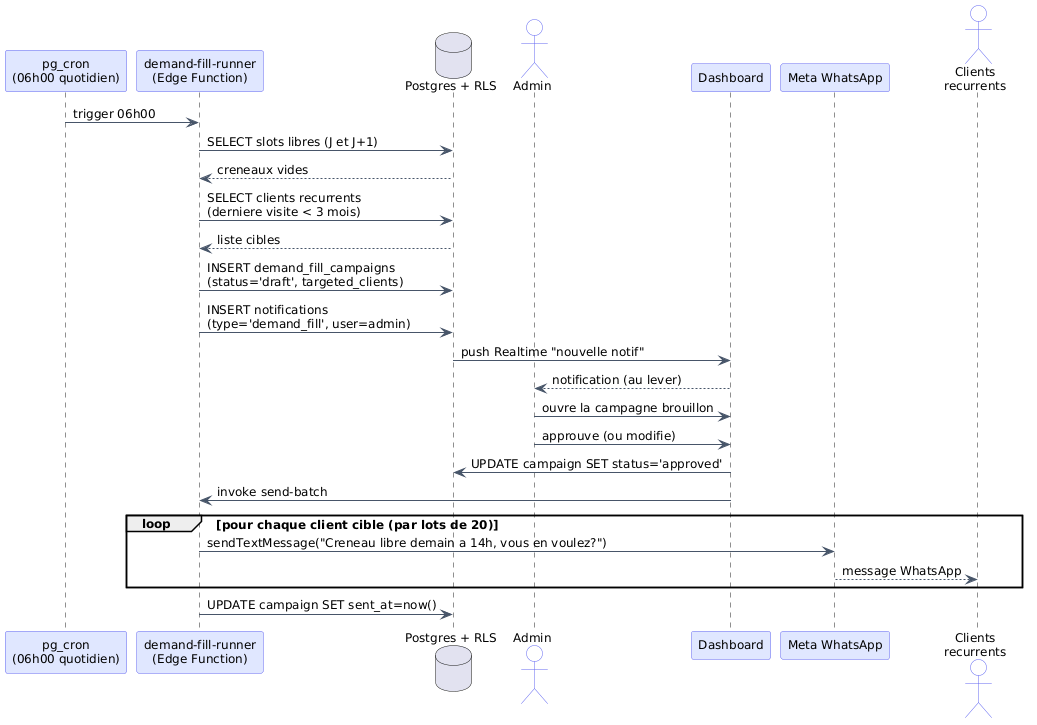
\includegraphics[width=.95\textwidth,height=.6\textheight,keepaspectratio]{figures/seq-s3-demand-fill.png}%
}{\fbox{\parbox[c][4cm][c]{.85\textwidth}{\centering\itshape\small[seq-s3-demand-fill.puml -- a generer via plantuml.com]}}}
\caption{Diagramme de séquence : Remplir créneaux vides (cron, brouillon, approbation admin, envoi par lots).}
\label{fig:seq-s3-fill}
\end{figure}

\paragraph{Générer voucher anniversaire.}
\begin{figure}[!htbp]\centering
\IfFileExists{figures/seq-s3-voucher.png}{%
  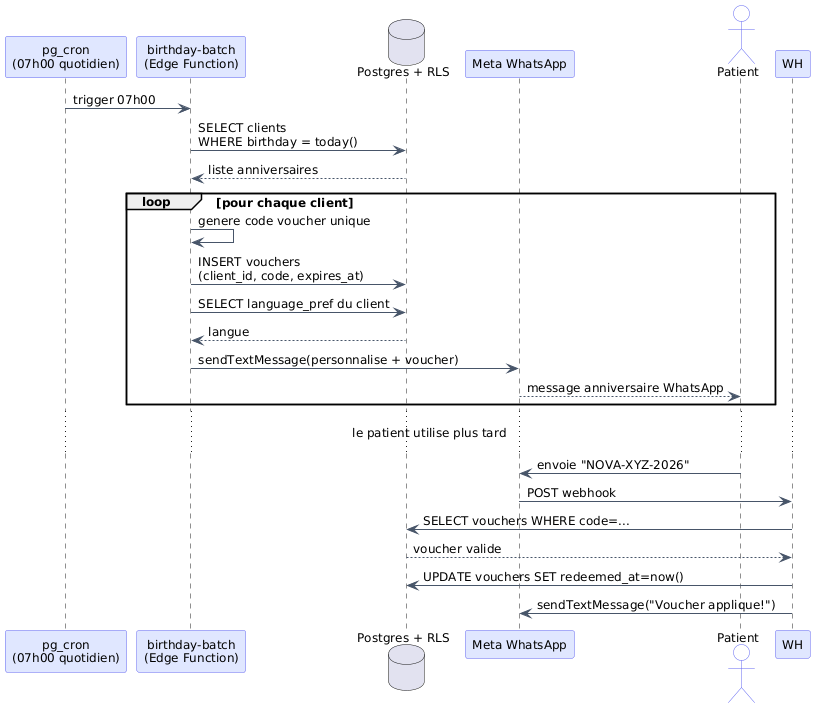
\includegraphics[width=.95\textwidth,height=.55\textheight,keepaspectratio]{figures/seq-s3-voucher.png}%
}{\fbox{\parbox[c][4cm][c]{.85\textwidth}{\centering\itshape\small[seq-s3-voucher.puml -- a generer via plantuml.com]}}}
\caption{Diagramme de séquence : Générer et envoyer voucher d'anniversaire WhatsApp, puis auto-rédemption.}
\label{fig:seq-s3-voucher}
\end{figure}

\paragraph{Scanner QR de réception (file d'attente temps réel).}
\begin{figure}[!htbp]\centering
\IfFileExists{figures/seq-s3-queue.png}{%
  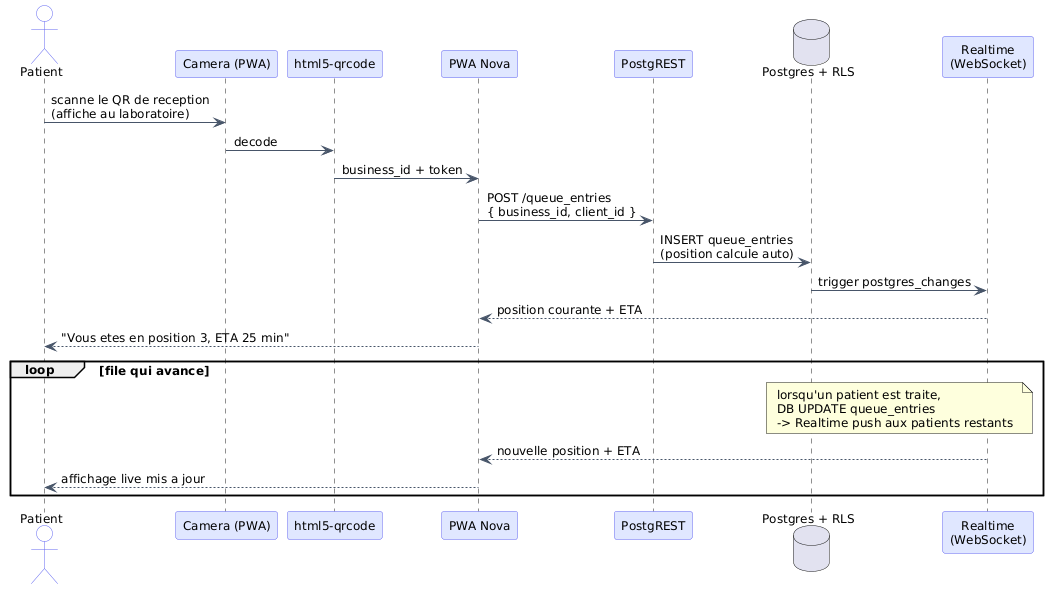
\includegraphics[width=.95\textwidth,height=.55\textheight,keepaspectratio]{figures/seq-s3-queue.png}%
}{\fbox{\parbox[c][4cm][c]{.85\textwidth}{\centering\itshape\small[seq-s3-queue.puml -- a generer via plantuml.com]}}}
\caption{Diagramme de séquence : Scanner QR de réception et suivre la position dans la file en temps réel (Realtime).}
\label{fig:seq-s3-queue}
\end{figure}

\section{Implémentation du Sprint 3}

\subsection{Surfaces administrateur étendues}
Le tableau de bord du Sprint~3 ajoute plusieurs surfaces~: gestion
des vouchers, approbation Demand-Fill, page Observation clinique
avec rapport de session, et paramètres avancés.

\begin{figure}[!htbp]\centering
\includegraphics[width=.95\textwidth,keepaspectratio]{figures/dashboard-qr-scan.jpg}
\caption{Scan QR patient depuis le tableau de bord administrateur.}
\label{fig:dash-qr}
\end{figure}

\begin{figure}[!htbp]\centering
\includegraphics[width=.95\textwidth,keepaspectratio]{figures/dashboard-observation.jpg}
\caption{Page Observation clinique : session en cours et historique.}
\label{fig:dash-observation}
\end{figure}

\begin{figure}[!htbp]\centering
\includegraphics[width=.95\textwidth,keepaspectratio]{figures/dashboard-observation-report.jpg}
\caption{Rapport de session : indicateurs, posture dominante, événements.}
\label{fig:dash-report}
\end{figure}

\begin{figure}[!htbp]\centering
\includegraphics[width=.95\textwidth,keepaspectratio]{figures/dashboard-settings.jpg}
\caption{Paramètres : voix clonée, fonctionnalités, working hours.}
\label{fig:dash-settings}
\end{figure}

\subsection{Surfaces patient enrichies (PWA)}
La PWA gagne des écrans dédiés~: assistant vocal \emph{Ask Nova},
catalogue de services consultable côté patient, et avatars
vocaux personnalisés.

\begin{figure}[!htbp]\centering
\includegraphics[width=.60\textwidth,keepaspectratio]{figures/mobile-voice.jpg}
\caption{Assistant vocal Ask~Nova depuis la PWA.}
\label{fig:pwa-voice}
\end{figure}

\begin{figure}[!htbp]\centering
\includegraphics[width=.55\textwidth,keepaspectratio]{figures/mobile-services.jpg}
\caption{PWA : catalogue de services consultable côté patient.}
\label{fig:pwa-services}
\end{figure}

\subsection{Avatars vocaux et observation patient}
La fonctionnalité d'avatars vocaux permet de cloner la voix de
l'administrateur (échantillon de trois minutes) via ElevenLabs,
puis de servir des messages personnalisés (rappels, vouchers) avec
sa voix réelle. L'observation patient utilise MediaPipe~Pose pour
extraire des \emph{landmarks} pendant la consultation~: agitation
moyenne, posture dominante et événements significatifs sont
sauvegardés en texte (aucune vidéo n'est conservée).

\begin{figure}[!htbp]\centering
\includegraphics[width=.95\textwidth,keepaspectratio]{figures/nova-voice.jpg}
\caption{Page Avatars vocaux : enregistrement de l'échantillon, statut du clonage.}
\label{fig:nova-voice}
\end{figure}

\section{Tests unitaires et revue du Sprint 3}
\begin{itemize}
  \item \textbf{Demand-Fill.} Marquer un créneau libre la veille,
        déclencher le cron, vérifier qu'un brouillon de campagne
        est créé et que la notification arrive en moins de cinq
        secondes.
  \item \textbf{Voucher anniversaire.} Régler la date
        d'anniversaire de trois clients de test à aujourd'hui,
        exécuter le batch, vérifier les trois messages WhatsApp et
        les codes voucher uniques.
  \item \textbf{Apprentissage durées.} Insérer 20 rendez-vous d'un
        même service avec durée réelle de 35~minutes vs déclarée
        30~minutes, vérifier qu'une suggestion à 35~min est
        générée.
  \item \textbf{File d'attente.} Scanner deux QR successifs,
        vérifier que les positions 1 et 2 s'affichent en temps
        réel sur les deux téléphones.
  \item \textbf{Voix clonée.} Envoyer un texte de rappel, vérifier
        que la voix générée diffère perceptiblement de la voix
        par défaut et correspond à l'échantillon fourni.
\end{itemize}

La revue de sprint avec mon encadrante a validé l'activation des
packs sectoriels (clinique, laboratoire, garage, salon) et la
robustesse des automatismes de fond (cron Demand-Fill, batch
anniversaire, apprentissage des durées).

\section{Conclusion}
Le Sprint~3 a complété \nova{} par sa couche d'intelligence~: le
produit ne se contente plus de réagir aux messages, il agit
proactivement (remplissage, anniversaires, durées) et propose des
expériences enrichies (voix clonée, observation, file d'attente
temps réel). Le chapitre suivant (Conclusion générale) revient sur
le bilan global du projet et ouvre les perspectives d'évolution.
